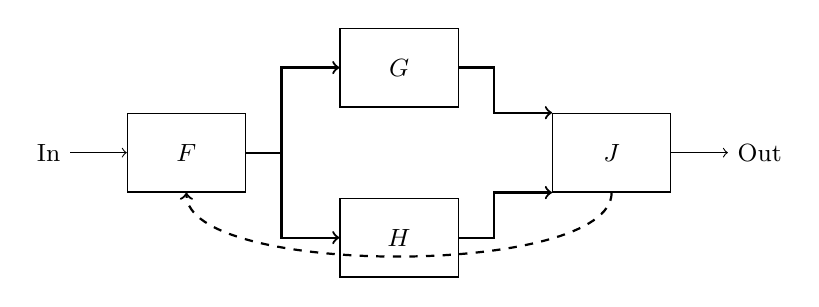
\begin{tikzpicture}[scale=0.9, every node/.style={font=\small}]
  % Boxes
  \node[draw, rectangle, minimum width=1.5cm, minimum height=1cm] (F) at (0,0) {$F$};
  \node[draw, rectangle, minimum width=1.5cm, minimum height=1cm] (G) at (3,1.2) {$G$};
  \node[draw, rectangle, minimum width=1.5cm, minimum height=1cm] (H) at (3,-1.2) {$H$};
  \node[draw, rectangle, minimum width=1.5cm, minimum height=1cm] (J) at (6,0) {$J$};

  % Wires
  \draw[->, thick] (F.east) -- ++(0.5,0) |- (G.west);
  \draw[->, thick] (F.east) -- ++(0.5,0) |- (H.west);
  \draw[->, thick] (G.east) -- ++(0.5,0) |- (J.north west);
  \draw[->, thick] (H.east) -- ++(0.5,0) |- (J.south west);

  % Feedback wire
  \draw[->, thick, dashed] (J.south) .. controls +(0,-1.2) and +(0,-1.2) .. (F.south);

  % Inputs/Outputs
  \draw[<-] (F.west) -- ++(-0.8,0) node[left] {In};
  \draw[->] (J.east) -- ++(0.8,0) node[right] {Out};
\end{tikzpicture}